\chapter{Perturbed system}
\label{perturbed}

So far, we have seen how to compute the dispersion relation for some simple
lattices. Now we want to see what sorts of effects we can create by introducing
some perturbations. We will do this in terms of changing the masses as well as
the spring constants between each mass in Chapter \ref{formbandgap}. Later on
in Chapter \ref{formstrip}, we will form a 2d strip or ribbon of these cells,
with the top half possessing one set of properties and the bottom half
possessing a different set of properties. We will see that this cause an
interesting phenomenon to occur at the boundary of the two halves.

\textit{Note}: As the hexagonal and kagome lattices contain more symmetries due
to the shape of their elementary cell, we will be focusing on perturbing these
models, but the same can be done for the square lattice as well. 

\section{Band gap}
\label{formbandgap}

\begin{figure}[!h]
\centering
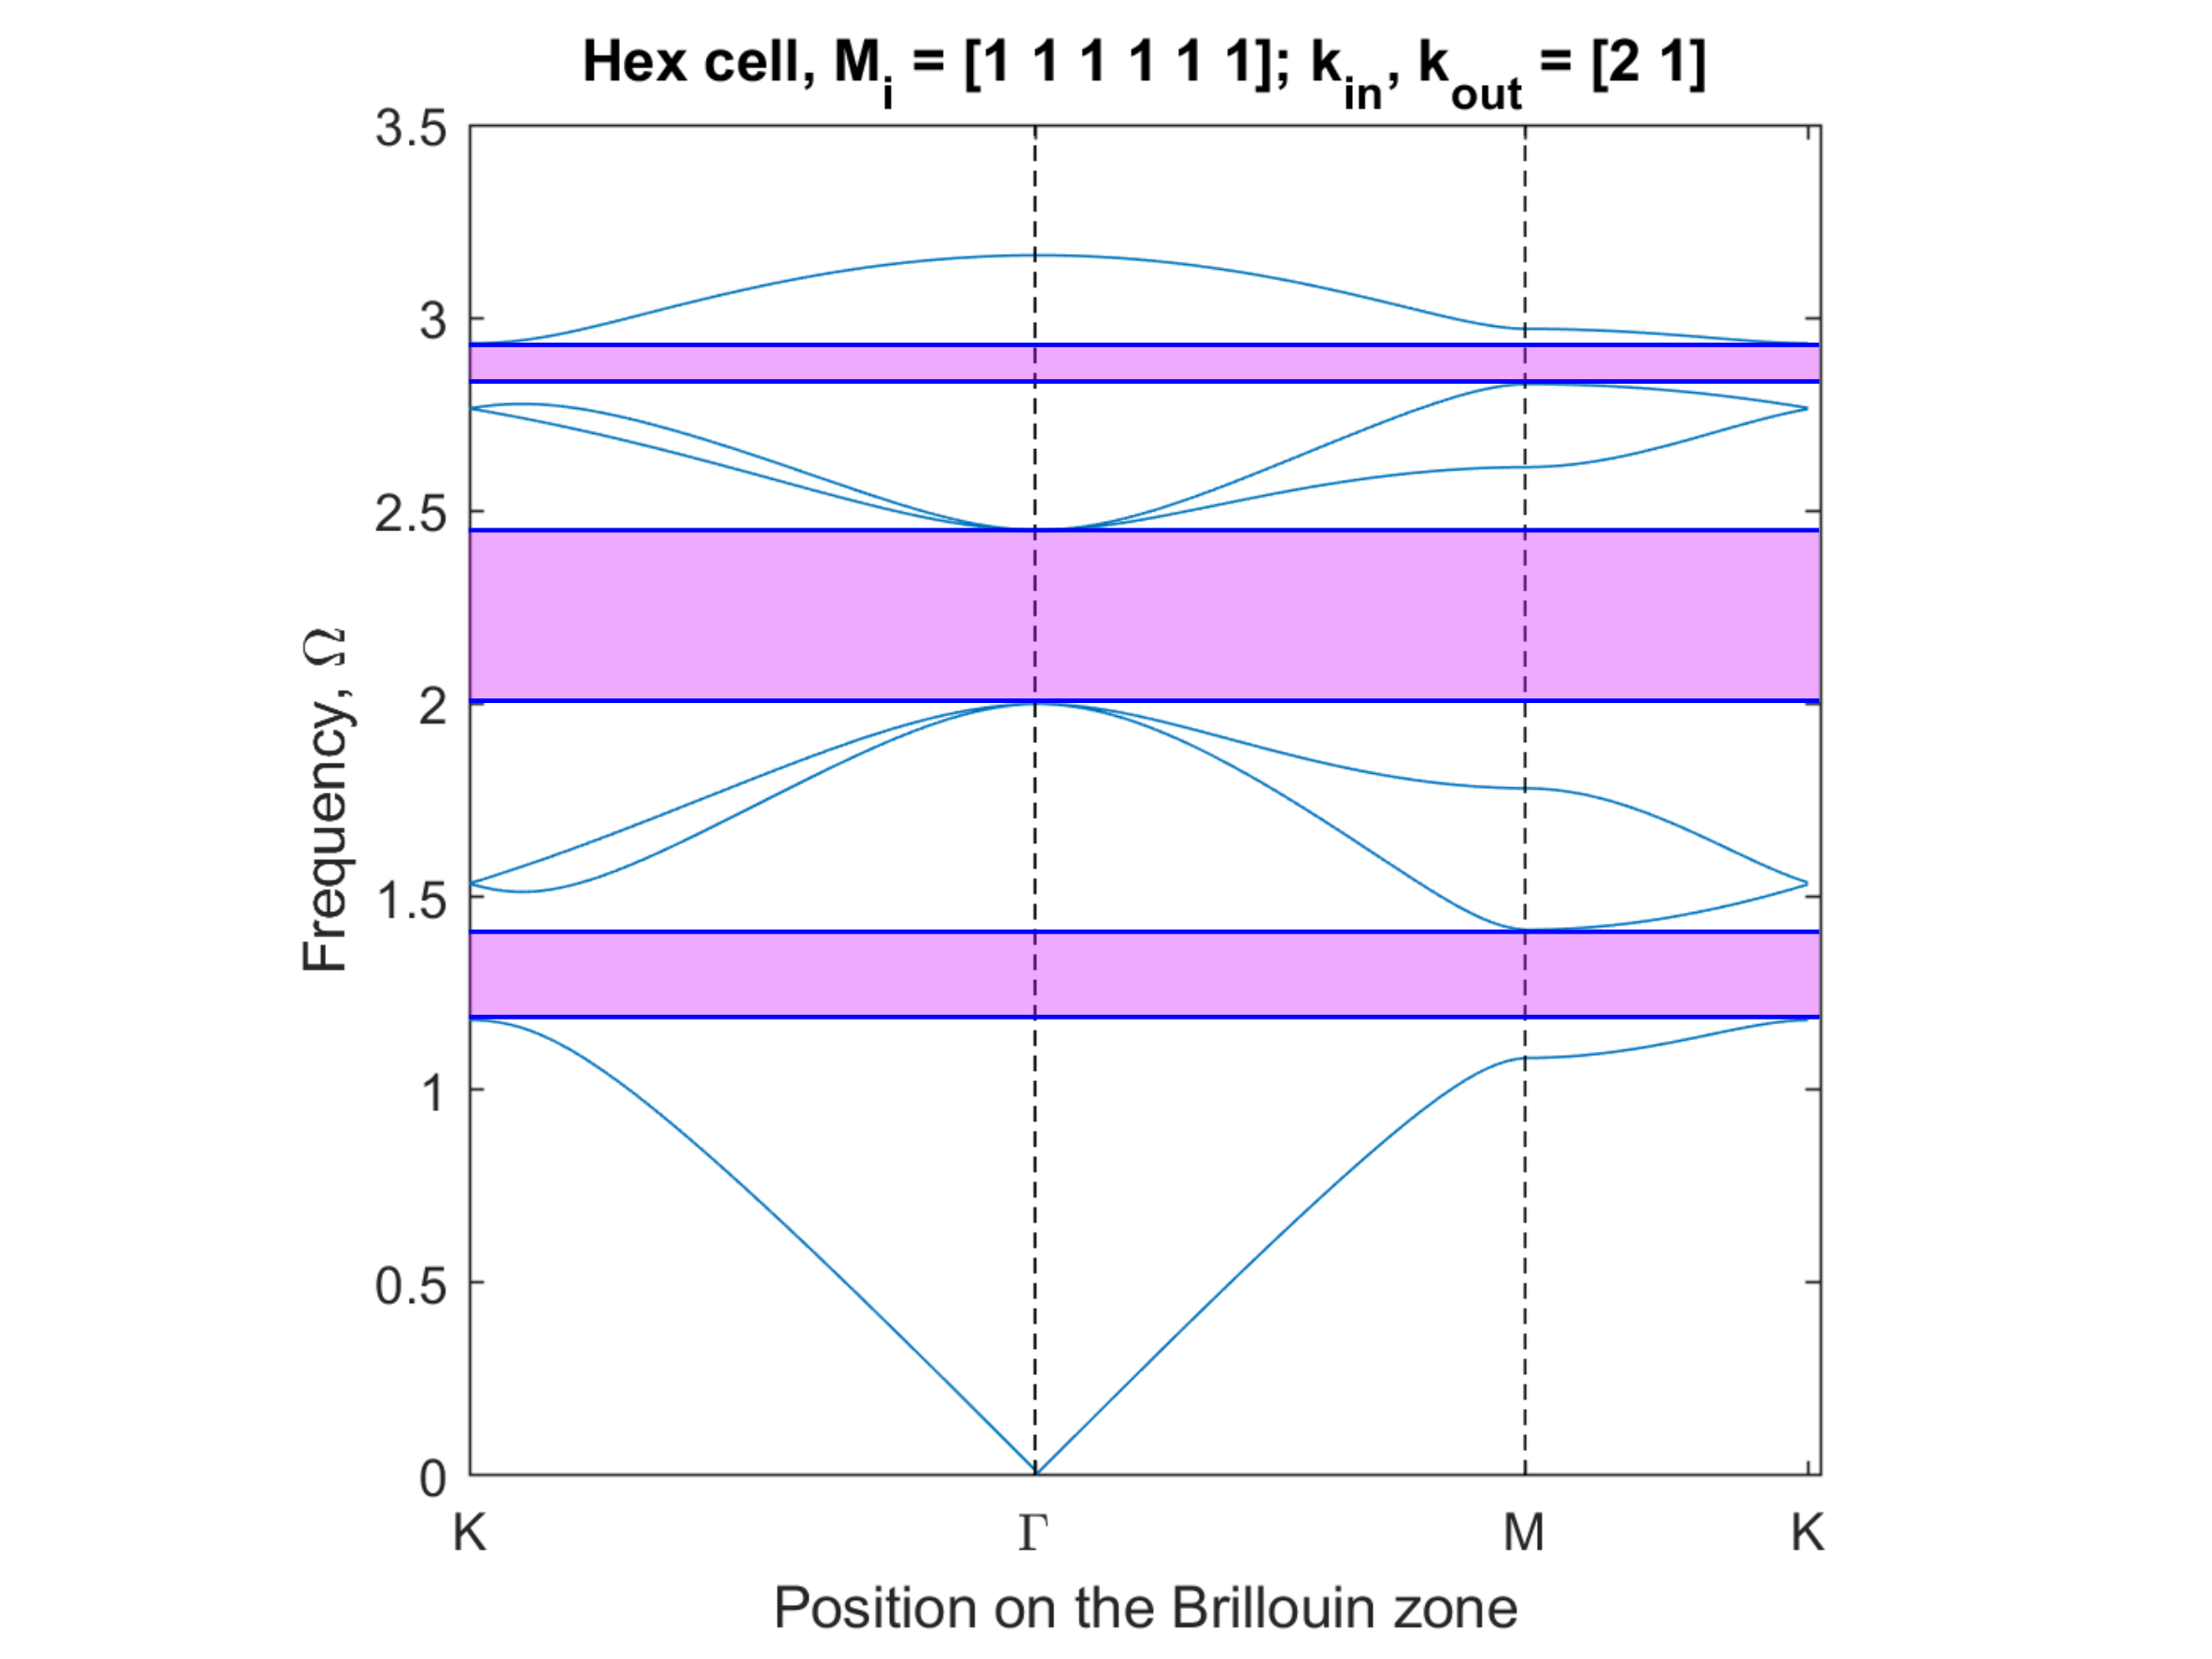
\includegraphics[width=0.8\textwidth]{imgs/bandgapex.png}
\caption{\label{fig:bandgapex} Example of bandgap (purple) formed in dispersion
  relation of hex lattice when $k=2$ and $\tilde{k}=1$.}
\end{figure}

A band gap, also called an energy gap, is an energy range where no wave states
can exist. In terms of our lattices, this corresponds to a range of frequencies
where waves are unable to propagate through the material; and in graphs of
dispersion relations, it is seen as gaps in the frequency axis where no line
is present. An example is shown in Figure~\ref{fig:bandgapex}. 
%TODO: What is a bandgap?

\section{2d bulk hexagonal perturbation}
Due to the many symmetries of the hexagonal lattice, there are many different
ways for us to perturb its structure and break its symmetry. These all lead to
slightly different effects on the dispersion relation.

\subsection{Alternating masses}
One way to perturb our bulk hexagonal lattice is by breaking one of its
rotational symmetries. Currently our hexagonal lattice has six-fold rotational
symmetry, i.e. rotating our cells by $\frac{2\pi}{6}$ do not change them. We can
reduce this to a three-fold symmetry by alternating the masses such that
$M_1=M_3=M_5 \neq M_2=M_4=M_6$.

\begin{figure}[!h]
\centering
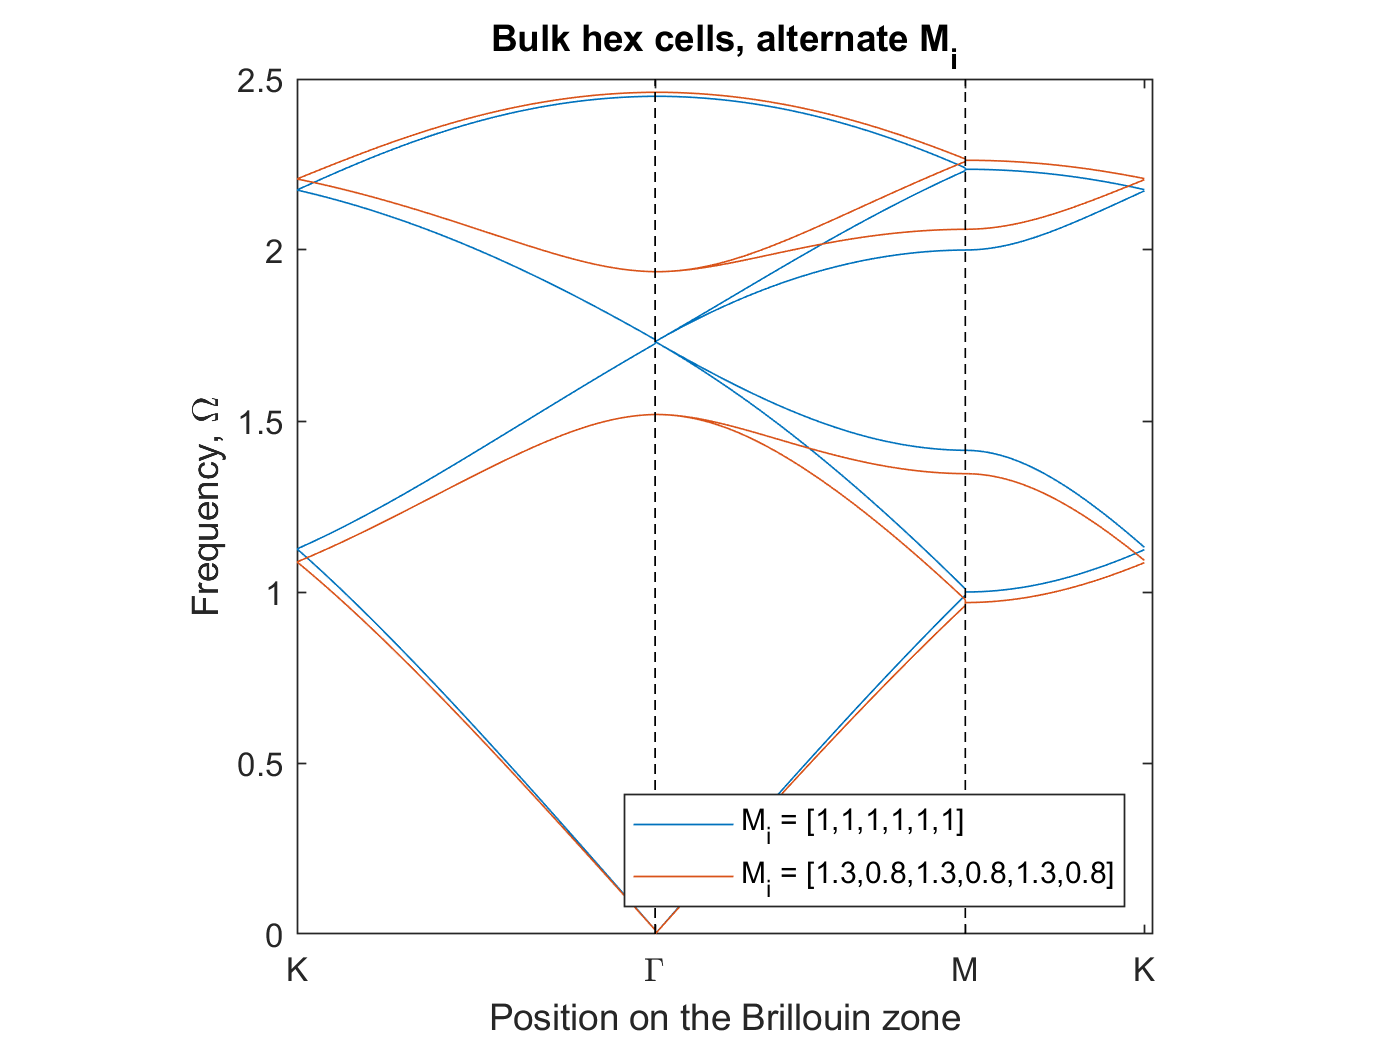
\includegraphics[width=0.8\textwidth]{imgs/hexperturbM.png}
\caption{\label{fig:hexM} The effect of alternating the masses $M_i$ on the
  dispersion relation of the bulk hexagonal system, with all other parameters
  set to $1$.}
\end{figure}

In Figure~\ref{fig:hexM}, we see that alternating masses has opened up the
double dirac point at $\Gamma$ and formed a bandgap.
%TODO: What is a dirac point?
%TODO: Add diagram showing rhombuses and how alternating has removed symmetry

\subsection{Varying mass and stiffnesses}
Another way we can induce a bandgap in our system is by changing the ratio of
the inner stiffness to the outer stiffness. This not only breaks one of the
local symmetries (local in the sense of the individual cell) but also breaks
one of the \textit{global} symmetries that we get. 

If you look at our hexagonal lattice and focus on the springs connecting our
masses, you can see that we have two different hexagons being formed, one
within each cell and also another between three adjacent cells meeting at a
vertex. When we have $k=\tilde{k}$, the inner and outer springs "tug" on the
masses the same amount, and so the two different hexagons we were talking about
before are of exactly the same proportions. However, when we modify our system
such that the inner stiffness is greater, say, than the outer stiffness, the
inner hexagons within each cell will be more "tightly pulled in" on itself and
in turn causing the outer hexagons to become bigger.
%TODO: Add figure to show the hexagon sizes changing

\begin{figure}[!h]
\centering
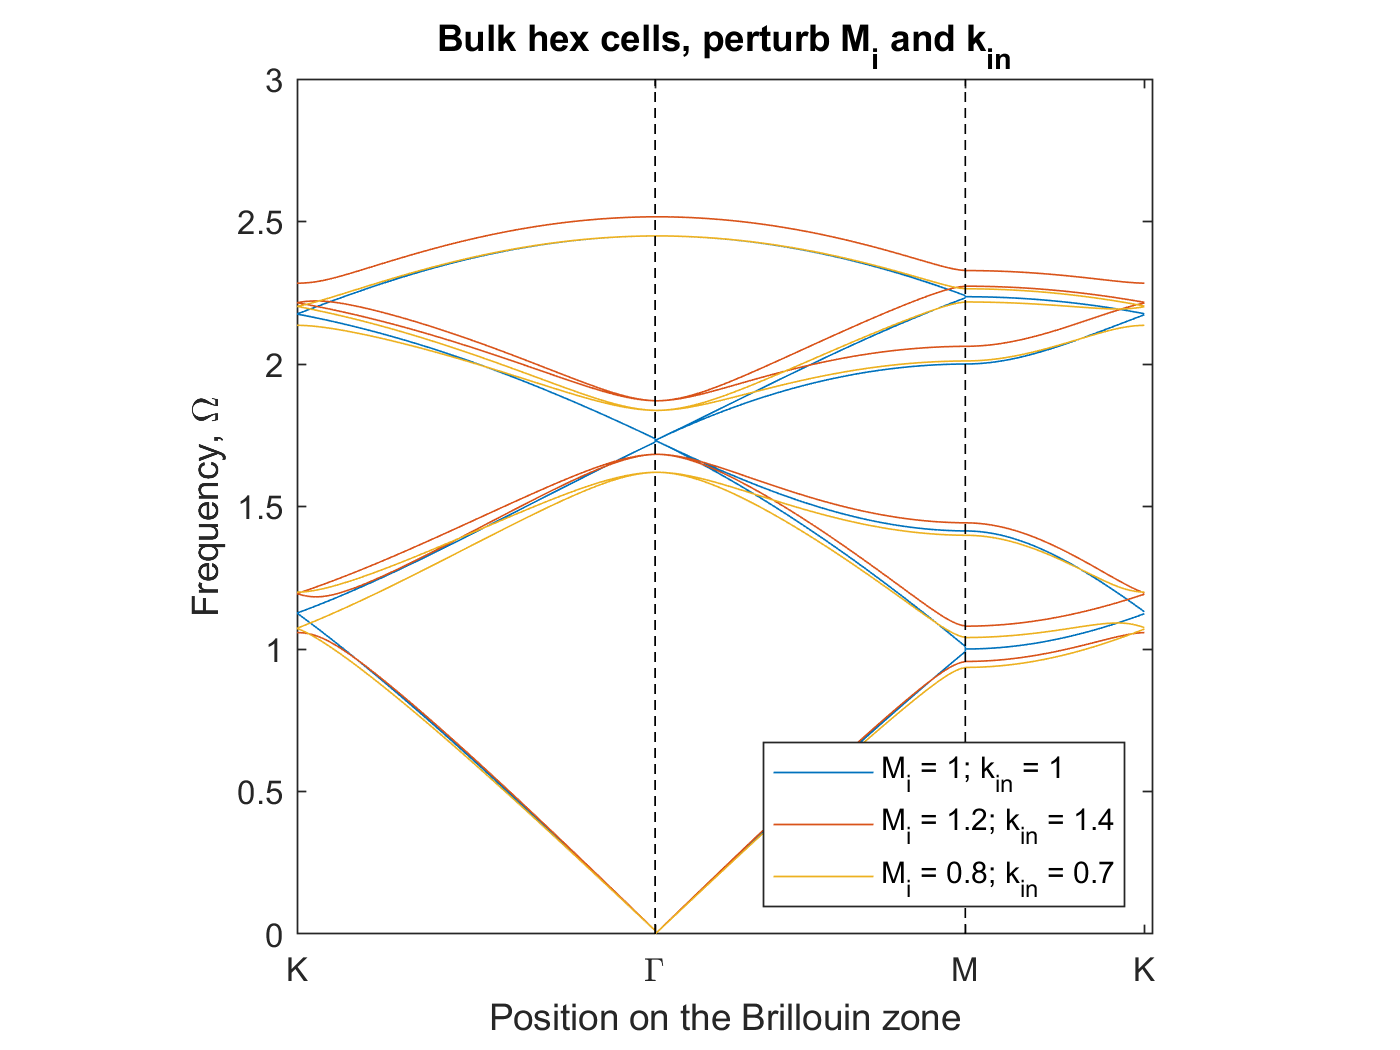
\includegraphics[width=0.8\textwidth]{imgs/hexperturb2.png}
\caption{\label{fig:hex2} The effect of perturbing the masses $M_i$ and
  $k$ on the dispersion relation of the bulk hexagonal system, with all other
  parameters set to $1$.}
\end{figure}

We can see in Figure~\ref{fig:hex2} that increasing both the mass and inner
stiffness as well as decreasing both the mass and inner stiffness leads to the
formation of a bandgap. Also notice that overall the magnitude of the bands are
about the same as the original bulk system we had. We take a closer look at how
changing $M_i$ and changing $k$ individually affect the dispersion relation in
the kagome lattice in Chapter \ref{kagomeperturb}.

%TODO: To include or not to include?
\section{2d hexagonal strip}
\label{formstrip}
%TODO: How does bandgap relate to the dispersion along the boundary?

\begin{figure}[!h]
\centering
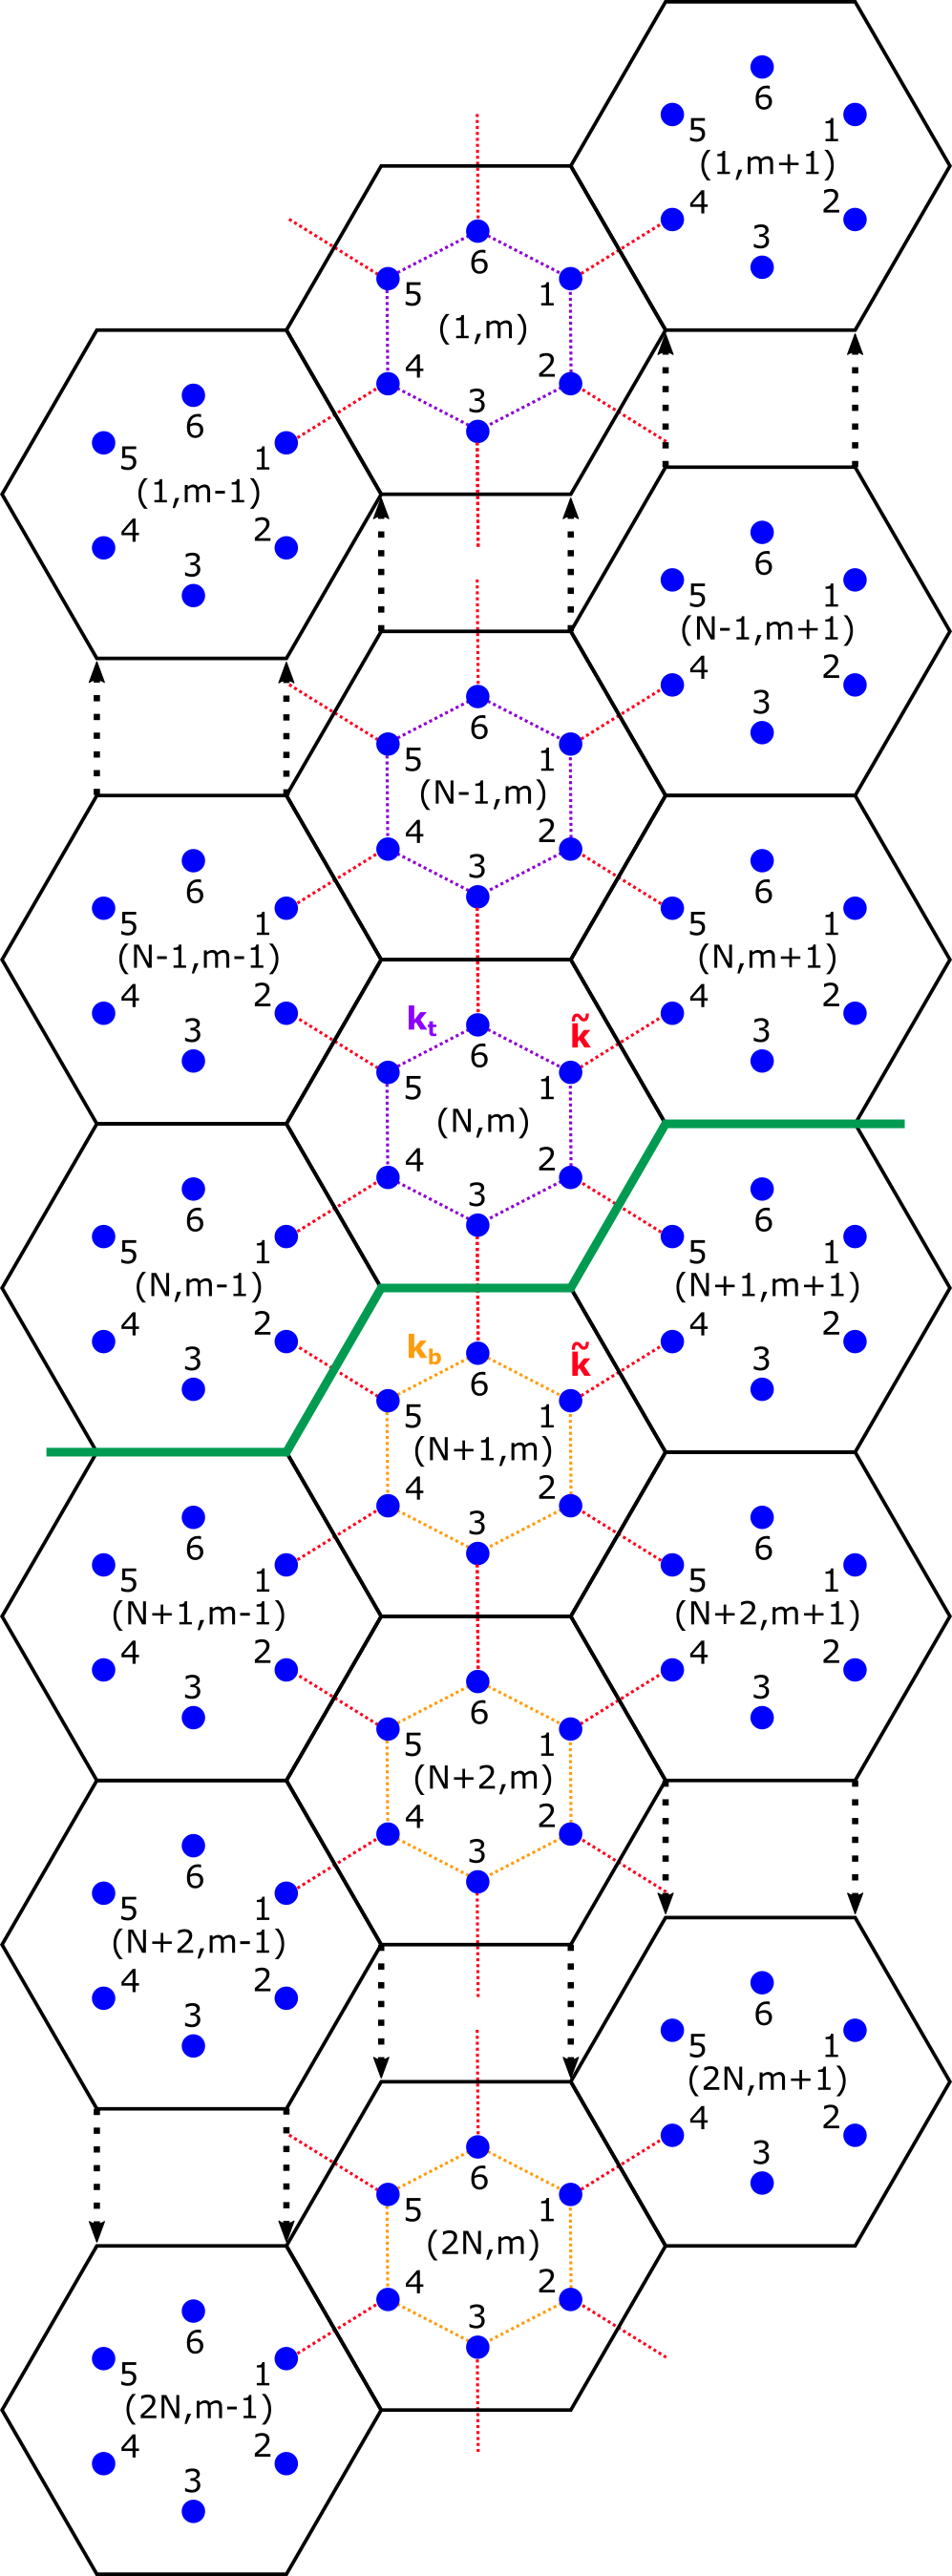
\includegraphics[width=0.4\textwidth]{imgs/hexstripmodel.png}
\caption{\label{fig:hexstripmodel} Schematic view of the 2d hexagonal
  semi-infinite lattice made from an infinite number of strips connected
  side-by-side. Each strip is composed of 2N cells, with the top half of cells
  above the boundary (green) possessing a set of properties and the bottom half
  possessing a separate set of properties. Note the the boundary conditions at
  the top and bottom, i.e. the cells at the top and bottom edges have no
  connections outside the lattice.}
\end{figure}

Now we assemble $2N$ hexagonal cells together into a strip and form a
semi-infinite hexagonal lattice by joining these strips from side-to-side as
shown in Figure~\ref{fig:hexstripmodel}. We will subscript the values
corresponding to the top half and bottom half with $t$ and $b$ respectively,
e.g. $k_t$ to refer to the inner spring constants for the top half and
$M_{1,b}$ to refer to the mass of mass $1$ in the bottom half. We set the outer
spring constant, $\tilde{k}_t=\tilde{k}_b=\tilde{k}$ to be the same throughout
the strip, to ensure that it agrees on both sides of the boundary or interface.

Using the same reasonings in Chapter \ref{2dhexdisper} to form equations
between adjacent cells, we can also form an eigen-problem as before (where the
size of our matrix is now $(2N \times 6) \times (2N \times 6)$ instead of $6
\times 6$). The only difference and extra care we have to take is to insert the
right coupling terms between masses in different cells, e.g. $M_3$ is not
connected to $M_6$ displaced by some phase shift anymore, but is connected to
$M_6$ in the cell below. 

Also, we explicitly choose the boundary condition where the top and bottom
cells have no connections outside the lattice. This is similar to having our
top and bottom edges connected to a \textit{rigid wall} as our waves are unable
to leave the lattice from those two edges. This is important to note as the
rigid boundary gives rise to a different dispersion curve at the top and bottom
boundaries which can lead to propagation of waves that we do not want, such as
in Figure~\ref{fig:kagomegentlebendscat}.

\textit{Note:} Another sensible periodic boundary condition which we could have
imposed at the top and bottom edges is by coupling the top and bottom cells
together across the edge. Specifically, we could impose

\begin{align}
  \matr{A}_{6,6(2N-1)+3}&=\matr{A}_{6(2N-1)+3,6}=-\tilde{k} \\
  \matr{A}_{5,6(2N-1)+2}&=-\tilde{k}e^{-i\Delta_1} \\
  \matr{A}_{6(2N-1)+2,5}&=-\tilde{k}e^{i\Delta_1} 
\end{align}

This essentially gives us an infinite lattice going from top to bottom, with
top and bottom materials alternating. Therefore essentially, the significant
difference which we will see between the two boundary conditions is that one
models the top and bottom edge as edges between our materials and a rigid wall,
and the other models the top and bottom edge as edges between our two
materials. However, we will see later on that this will not matter too much for
our scattering simulations as we will be exciting waves of frequencies in our
bandgaps. So if we take $N$ to be large enough, the exponential decay of the
wavefunctions across the strip is great enough to ensure our wave does not
propagate to the top and bottom edges anyways.

With that out of the way, we can finally form the eigen-problem

\begin{align}
  \left[\matr{A}\left(\kappa_{x},\kappa_{y}\right)-\matr{\Omega}\matr{M}\right]\vec{y}=\vec{0}
\label{eq:hexstripeig}
\end{align}

where $\matr{A}$ is a $(2N \times 6) \times (2N \times 6)$ matrix with
$\matr{A}$ as defined in \eqref{eq:hexeig} repeated along the diagonal and with
the additional coupling terms added,
$\matr{\Omega}=\diag\left(\left\{\Omega_i^2\right\}\right)$,
$\matr{M}_{t}=\diag\left(\left\{M_{i,t}\right\}\right)$,
$\matr{M}_{b}=\diag\left(\left\{M_{i,b}\right\}\right)$,
\begin{align}
\matr{M}=\left[
\begin{array}{cccccc}
\matr{M}_{t}\\
 & \ddots &  &  & 0\\
 &  & \matr{M}_{t}\\
 &  &  & \matr{M}_{b}\\
 & 0 &  &  & \ddots\\
 &  &  &  &  & \matr{M}_{b}
\end{array}\right],
\end{align}

\begin{align}
\vec{y}=\left[
\begin{array}{c}
y_1^{(1)}\\
\vdots\\
y_6^{(1)}\\
\vdots\\
y_1^{(2N)}\\
\vdots\\
y_6^{(2N)}\\
\end{array}\right],
\end{align}

Now with this eigen-problem, all we have left to do is figure out what the
irreducible Brillouin zone for our ribbon system is.
%TODO: Add derivation of IBZ for hexagonal ribbon system

Solving this with $M_{i,t}=M_{i,b}=k_t=k_b=\tilde{k}=1$ over the irreducible
Brilloun zone gives us the dispersion relation in
Figure~\ref{fig:hexstripdisper}, which corresponds to what we see in
Figure~\ref{fig:hexdisper} (if you take the graph from $K$ to $\Gamma$ and then
reflect it about the vertical at $\Gamma$).

\begin{figure}[!h]
\centering
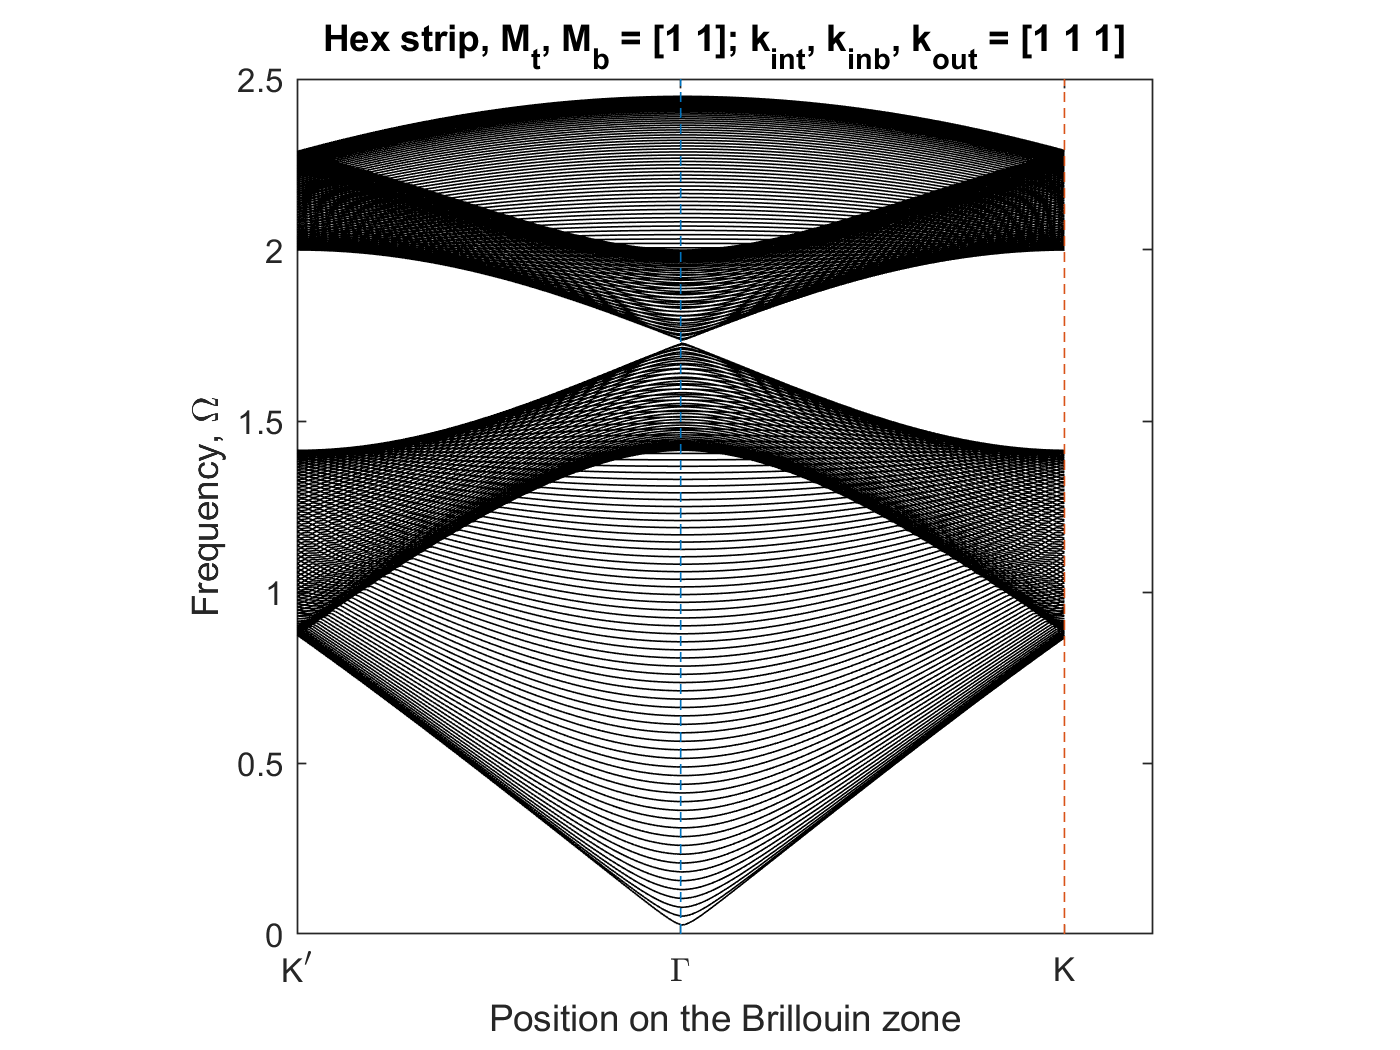
\includegraphics[width=0.8\textwidth]{imgs/hexstrip.png}
\caption{\label{fig:hexstripdisper} Dispersion relation of the semi-infinite
  hexagonal lattice with $2N=40$ (40 cells in total) with
  $M_{i,t}=M_{i,b}=k_t=k_b=\tilde{k}=1$.}
\end{figure}

As we have just done in Chapter \ref{formstrip}, we will see what happens to
the dispersion relation when we set the two layers of the lattice to have
different properties as those before which opened up a band gap.

\subsection{Alternating masses}
\label{perturbaltmass}
Using our results of the formation of a bandgap in, let us first see what
happens when we create a hexagonal strip where the top and bottom have the same
property of alternating masses. 

\begin{figure}[!h]
\centering
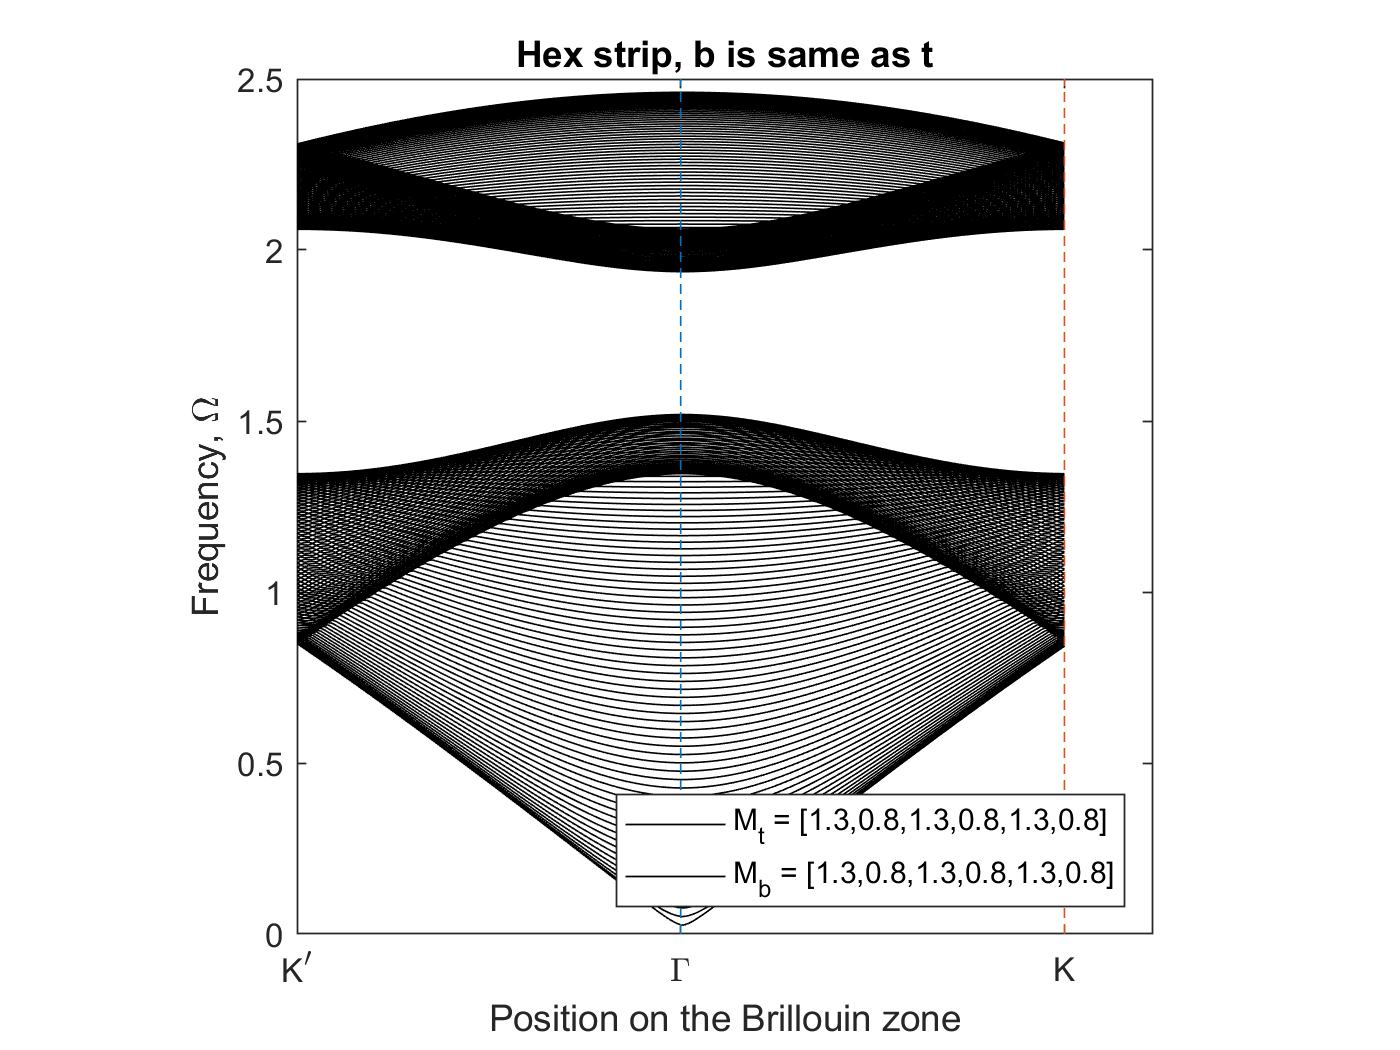
\includegraphics[width=0.8\textwidth]{imgs/hexstripperturbM.png}
\caption{\label{fig:hexstripM} Dispersion relation of the semi-infinite
  hexagonal lattice with alternating masses (with the top and bottom layer the
  same configuration), with all other parameters set to $1$.}
\end{figure}

Again, we see in Figure~\ref{fig:hexstripM} that basically the dispersion
relation we get corresponds to that of Figure~\ref{fig:hexM} (if you look at
the graph from $K$ to $\Gamma$ and reflect about $\Gamma$), where there is a
bandgap present. This is all fine and good but we can do something even better.

In this system, the two layers of materials are the same which means that
essentially it behaves just like the bulk hexagon case. It is as if we just
took a finite chunk of the infinite bulk lattice. So with that in mind, let us
change the bottom layer into a different configuration. The easiest way of
perturbing it so that we still get the exact same dispersion relation in the
bulk case is to rotate the cell by $\frac{2\pi}{6}$. This is because locally
(at the cellular level), nothing has changed and if we form a bulk system from
the rotated cell we still get the same bulk system but rotated, but this does
not affect the frequencies of waves allowed to propagate. So even if we stack
the two different types of cells on each other, we would expect the same
bandgap to be present, since locally each cell exhibits that property. However
if we now consider the global symmetry when stacking the two different
materials on top of each other, we can see that we have broken some sort of
translational symmetry and so would expect something different in the
dispersion relation.

\begin{figure}[!h]
\centering
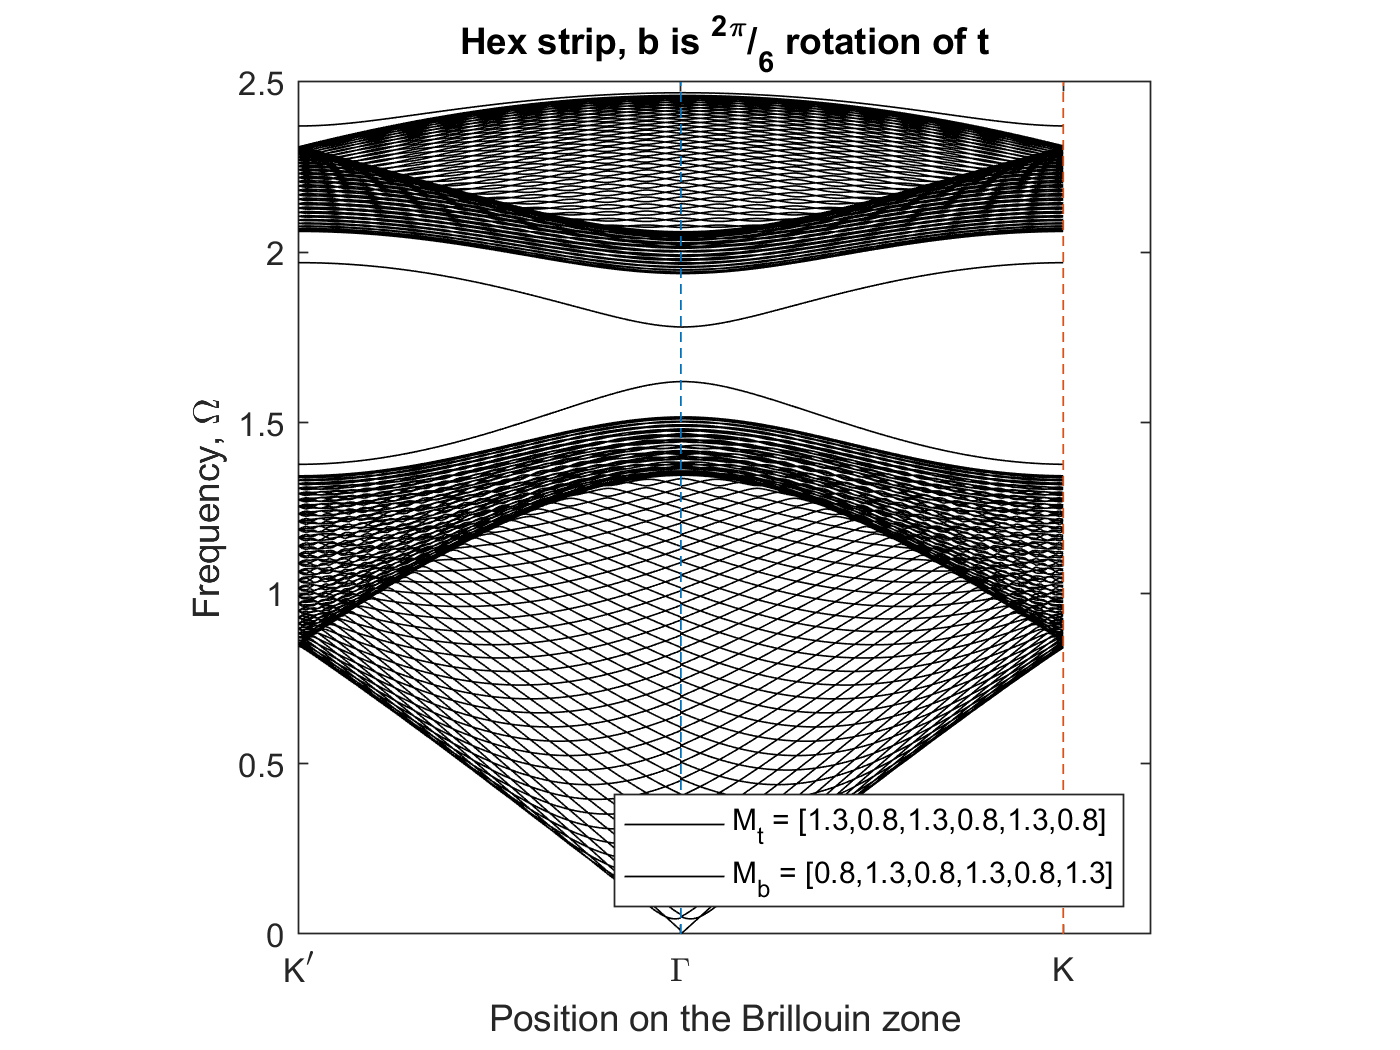
\includegraphics[width=0.8\textwidth]{imgs/hexstripperturbMrotated.png}
\caption{\label{fig:hexstripMrotated} Dispersion relation of the semi-infinite
  hexagonal lattice with alternating masses (with bottom layer as a
  $\frac{2\pi}{6}$ rotation of the top layer), with all other parameters set to
  $1$.}
\end{figure}

As expected, we see that in Figure~\ref{fig:hexstripMrotated} we get pretty
much the same dispersion relation as in Figure~\ref{fig:hexstripM} but with two
curious lines in the bandgap! This is really interesting and useful for us
because this means that all the frequencies along the two lines in the bandgap
are only able to propagate along the centre line of the semi-infinite lattice
we constructed, i.e. along the boundary and not anywhere else in the lattice.
The waves corresponding to the waves of these special frequencies are known as
the edge modes or edge states of our system, as they travel \textit{along the
edge} or boundary and exponentially decay outwards from that edge. With this
knowledge, we are then able to start trying to force energy to propagate in the
directions we desire in Chapter \ref{scattering}.
%TODO: How do we know it exponentially decays??
%TODO: Discuss the difference between the two lines, due to the periodic
%boundaries, one refers to the red over blue boundary, the other refers to blue
%over red

\subsection{Varying mass and stiffnesses}
\label{perturbMk}
We can do the same thing in this case, but instead of making the bottom layer a
rotation of the top layer, we make the top have a greater $M_i$ and $k$ and the
bottom have a lower $M_i$ and $k$. As we have seen in
Figure~\ref{fig:hex2}, we have one increased and one decreased system which
have similar bandgaps. As such, we will be using those two configurations to
form our strip.

\begin{figure}[!h]
\centering
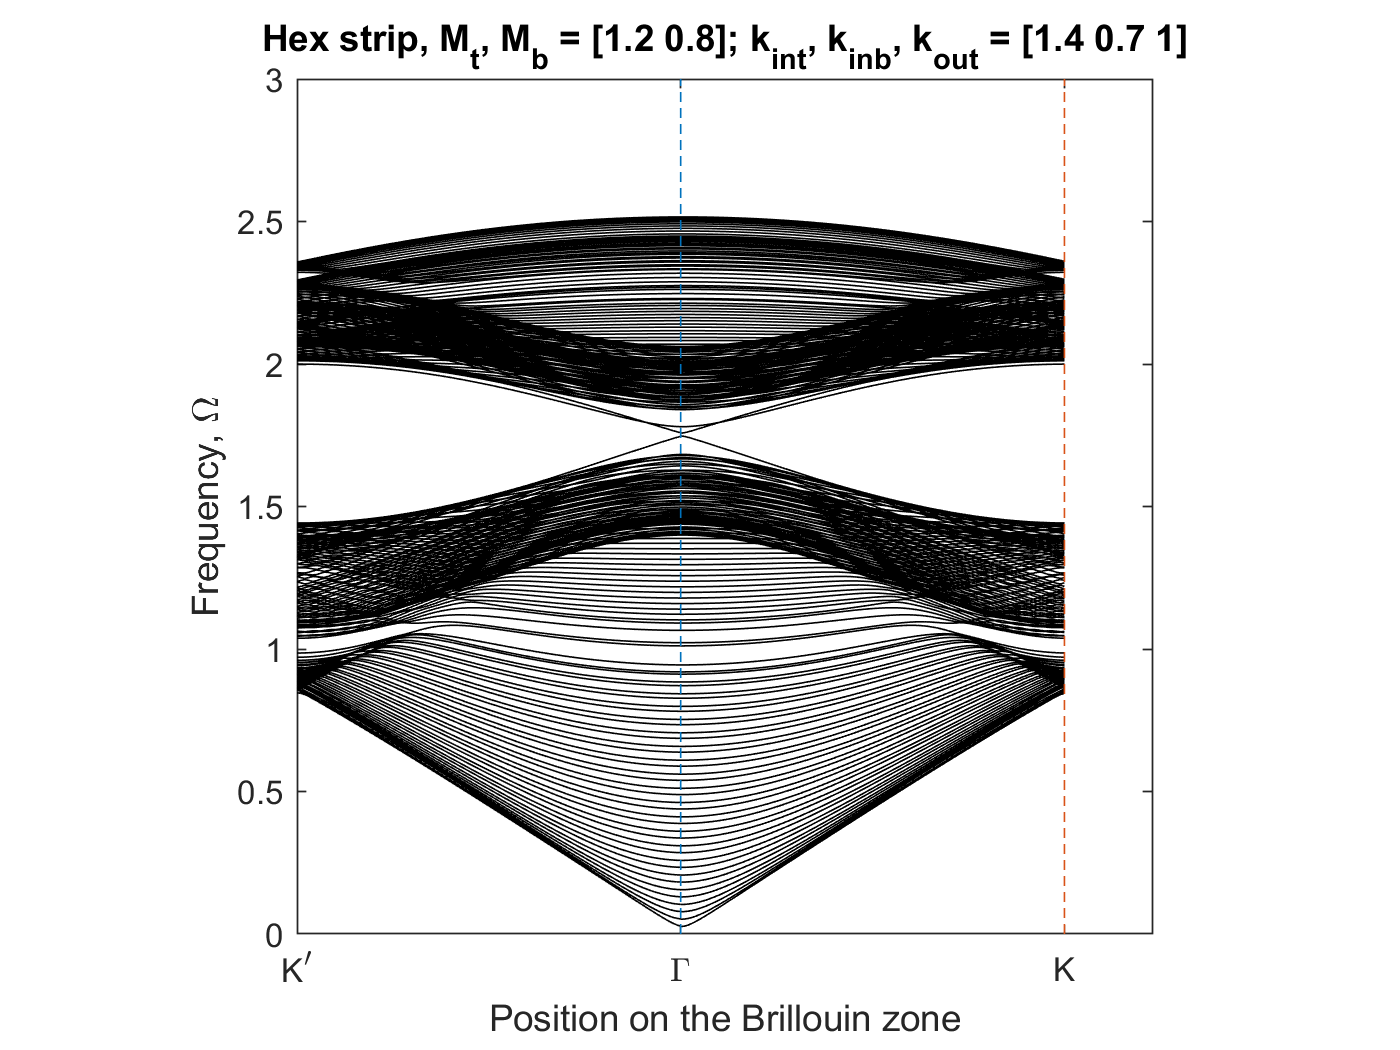
\includegraphics[width=0.8\textwidth]{imgs/hexstripperturb2.png}
\caption{\label{fig:hexstrip2} Dispersion relation of the semi-infinite
  hexagonal lattice where the top material has a higher $M_i$ and $k$ than the
  bottom material, with all other parameters set to $1$.}
\end{figure}

As before we again get a well-defined bandgap, as well as two dispersion lines
which are present in the bandgap and therefore correspond to edge states.

\section{2d bulk kagome perturbation}
\label{kagomeperturb}

Similarly to the hexagonal case, we can perturb the different parameters in our
bulk kagome system to see what effects they have on the dispersion relation.

\begin{figure}[!h]
\centering
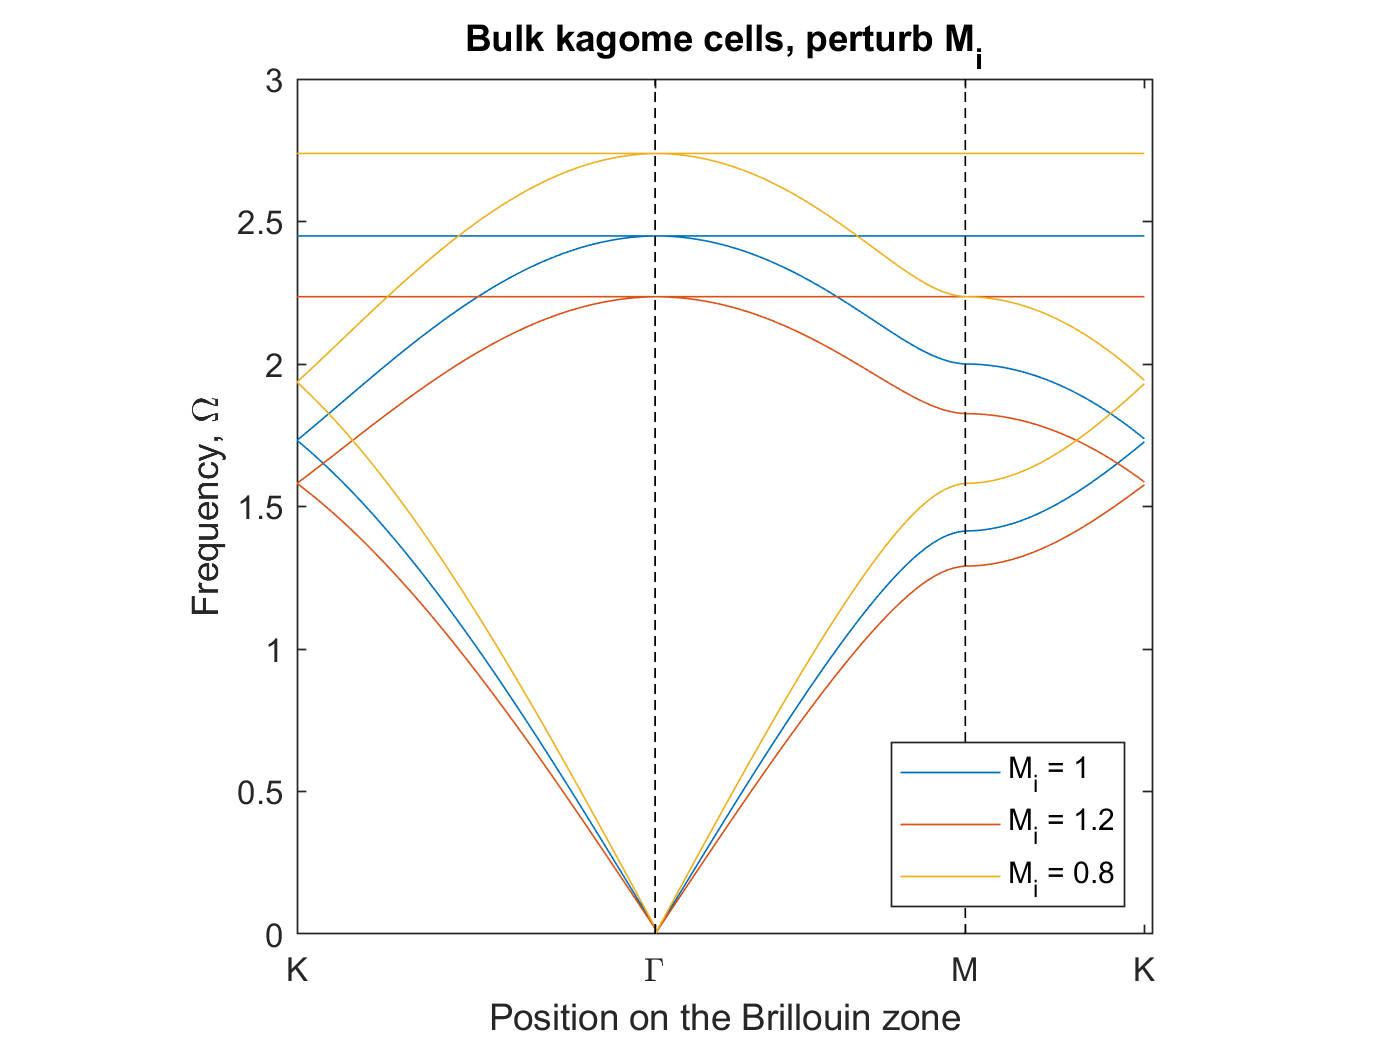
\includegraphics[width=0.8\textwidth]{imgs/kagomeperturbM.png}
\caption{\label{fig:kagomeM} The effect of perturbing the masses $M_i$ on the
  dispersion relation of the bulk kagome system, with all other parameters set
  to $1$.}
\end{figure}

\begin{figure}[!h]
\centering
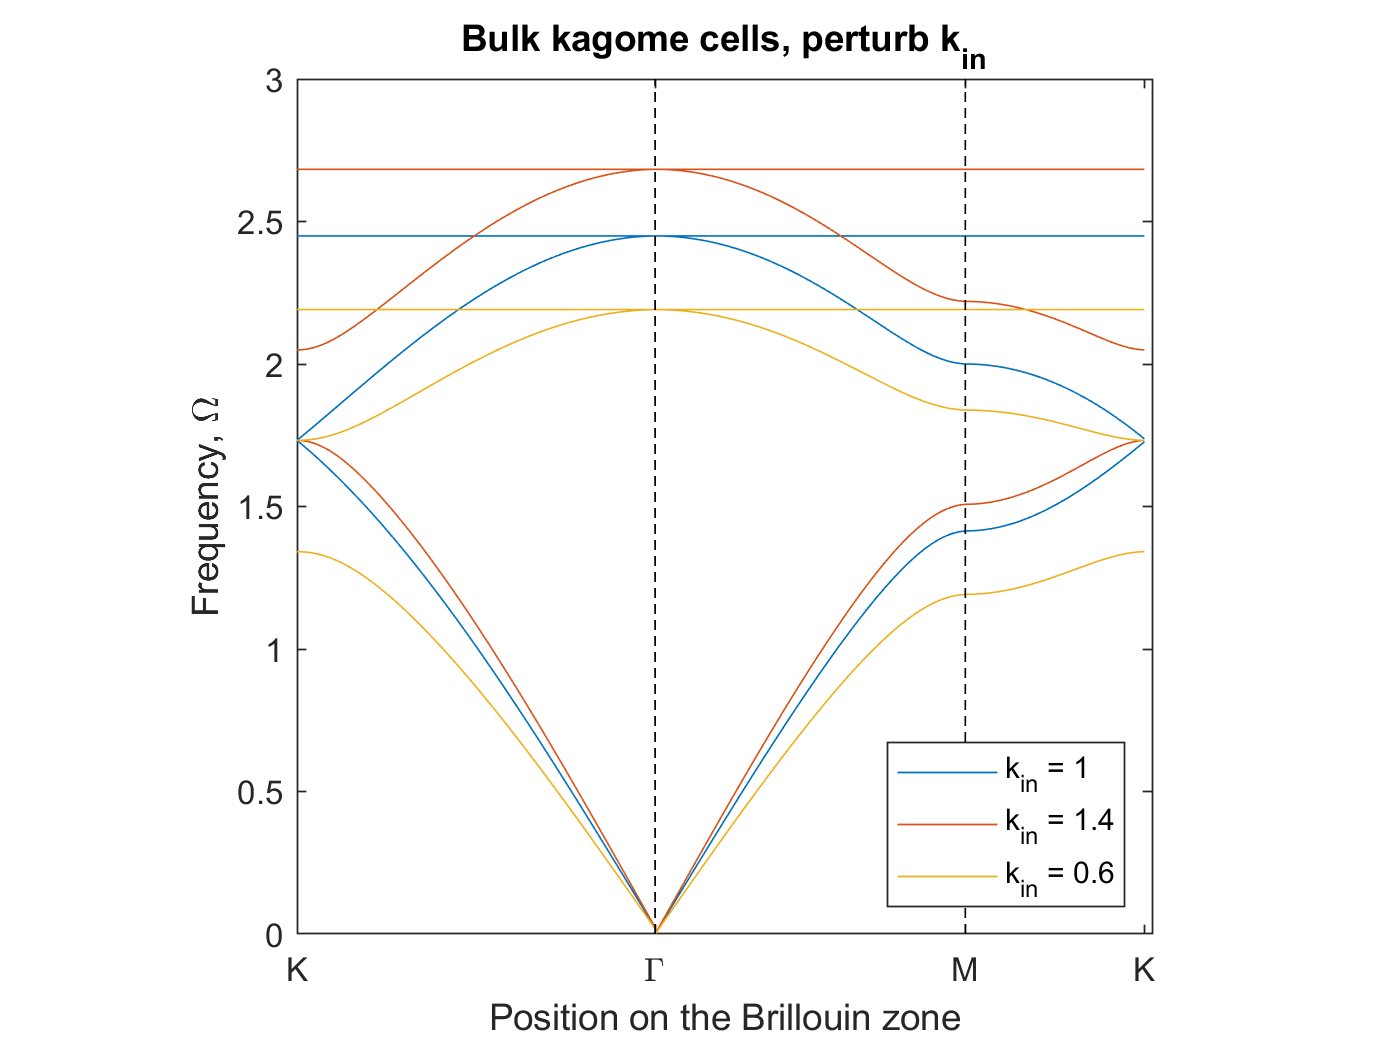
\includegraphics[width=0.8\textwidth]{imgs/kagomeperturbk.png}
\caption{\label{fig:kagomek} The effect of perturbing the inner stiffness $k$
  on the dispersion relation of the bulk kagome system, with all other
  parameters set to $1$.}
\end{figure}

We can see the effects that perturbing the masses $M_i$ and inner stiffness $k$
have on the bulk kagome system. In the case of varying $M_i$ in
Figure~\ref{fig:kagomeM}, increasing $M_i$ decreases or constrains the
dispersion relation, while decreasing $M_i$ increases or widens the dispersion
relation. 

However, in the case of varying $k$ in Figure~\ref{fig:kagomek}, we see the inverse
effect; increasing $k$ increases or widens the dispersion relation, while
decreasing $k$ decreases or constrains the dispersion relation. Another
interesting thing to notice about changing $k$ is that it causes the formation
of a bandgap!

With these two inverse relationships, we are naturally propelled to ask what
happens if we combine both of these effects together. For example, by
increasing $M_i$ and increasing $k$, would the two effects \textit{cancel out}
to give us the same dispersion relation as the unperturbed system? That is
precisely what happens and can be seen in Figure~\ref{fig:kagome2} as well as
Figure~\ref{fig:hex2}.

\begin{figure}[!h]
\centering
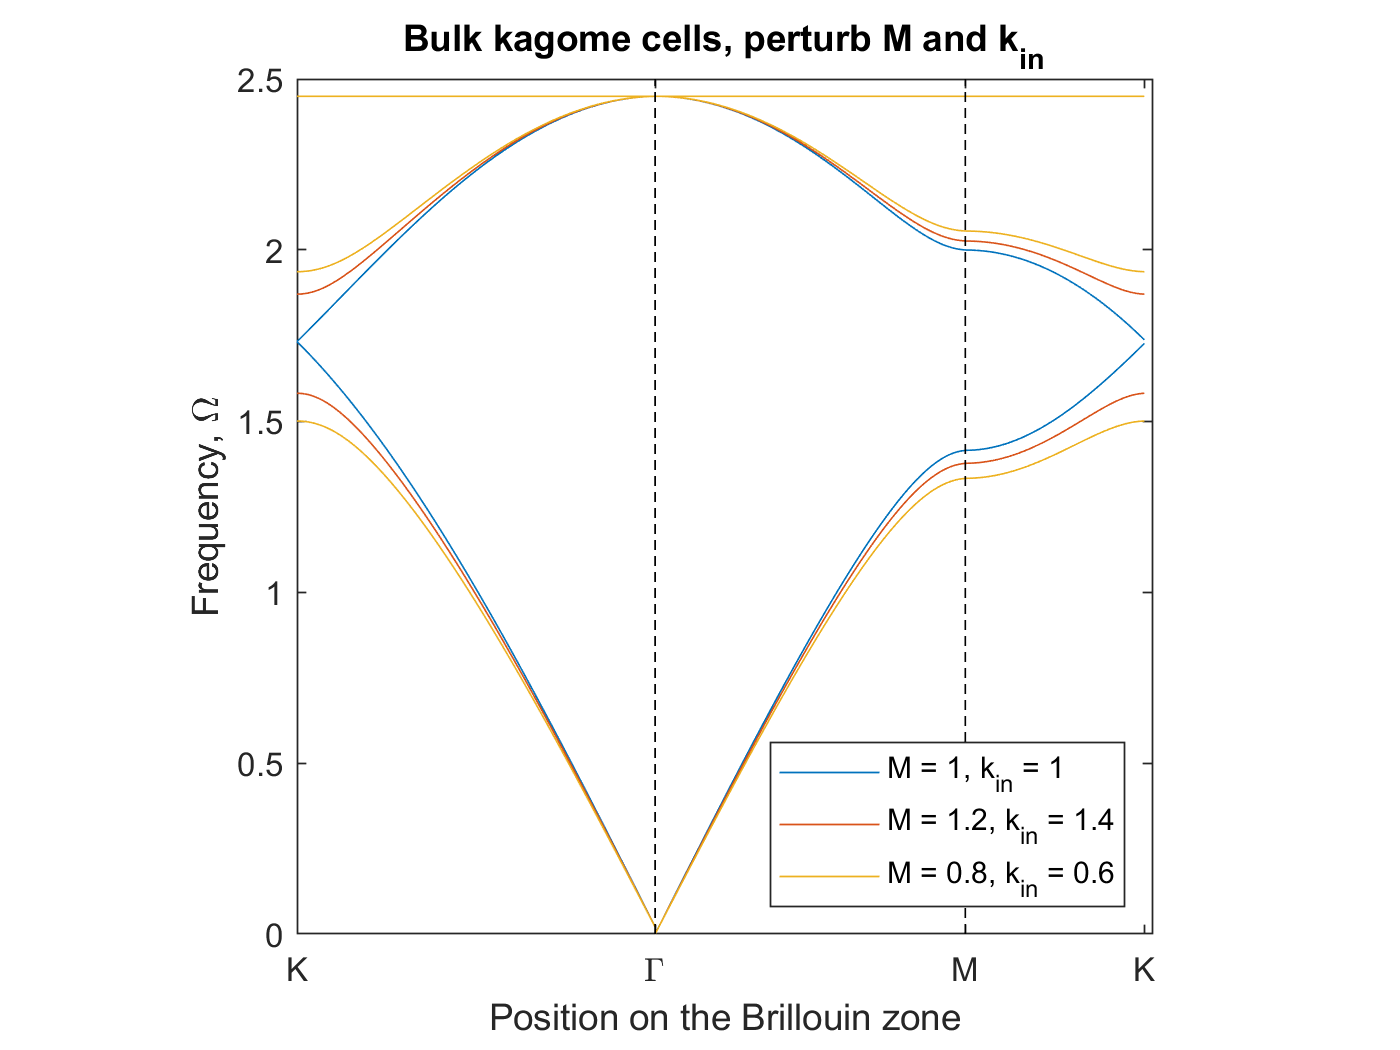
\includegraphics[width=0.8\textwidth]{imgs/kagomeperturb2.png}
\caption{\label{fig:kagome2} The effect of perturbing both the masses $M_i$ and
  the inner stiffness $k$ on the dispersion relation of the bulk kagome system,
  with all other parameters set to $1$.}
\end{figure}

\section{2d kagome strip}

\begin{figure}[!h]
\centering
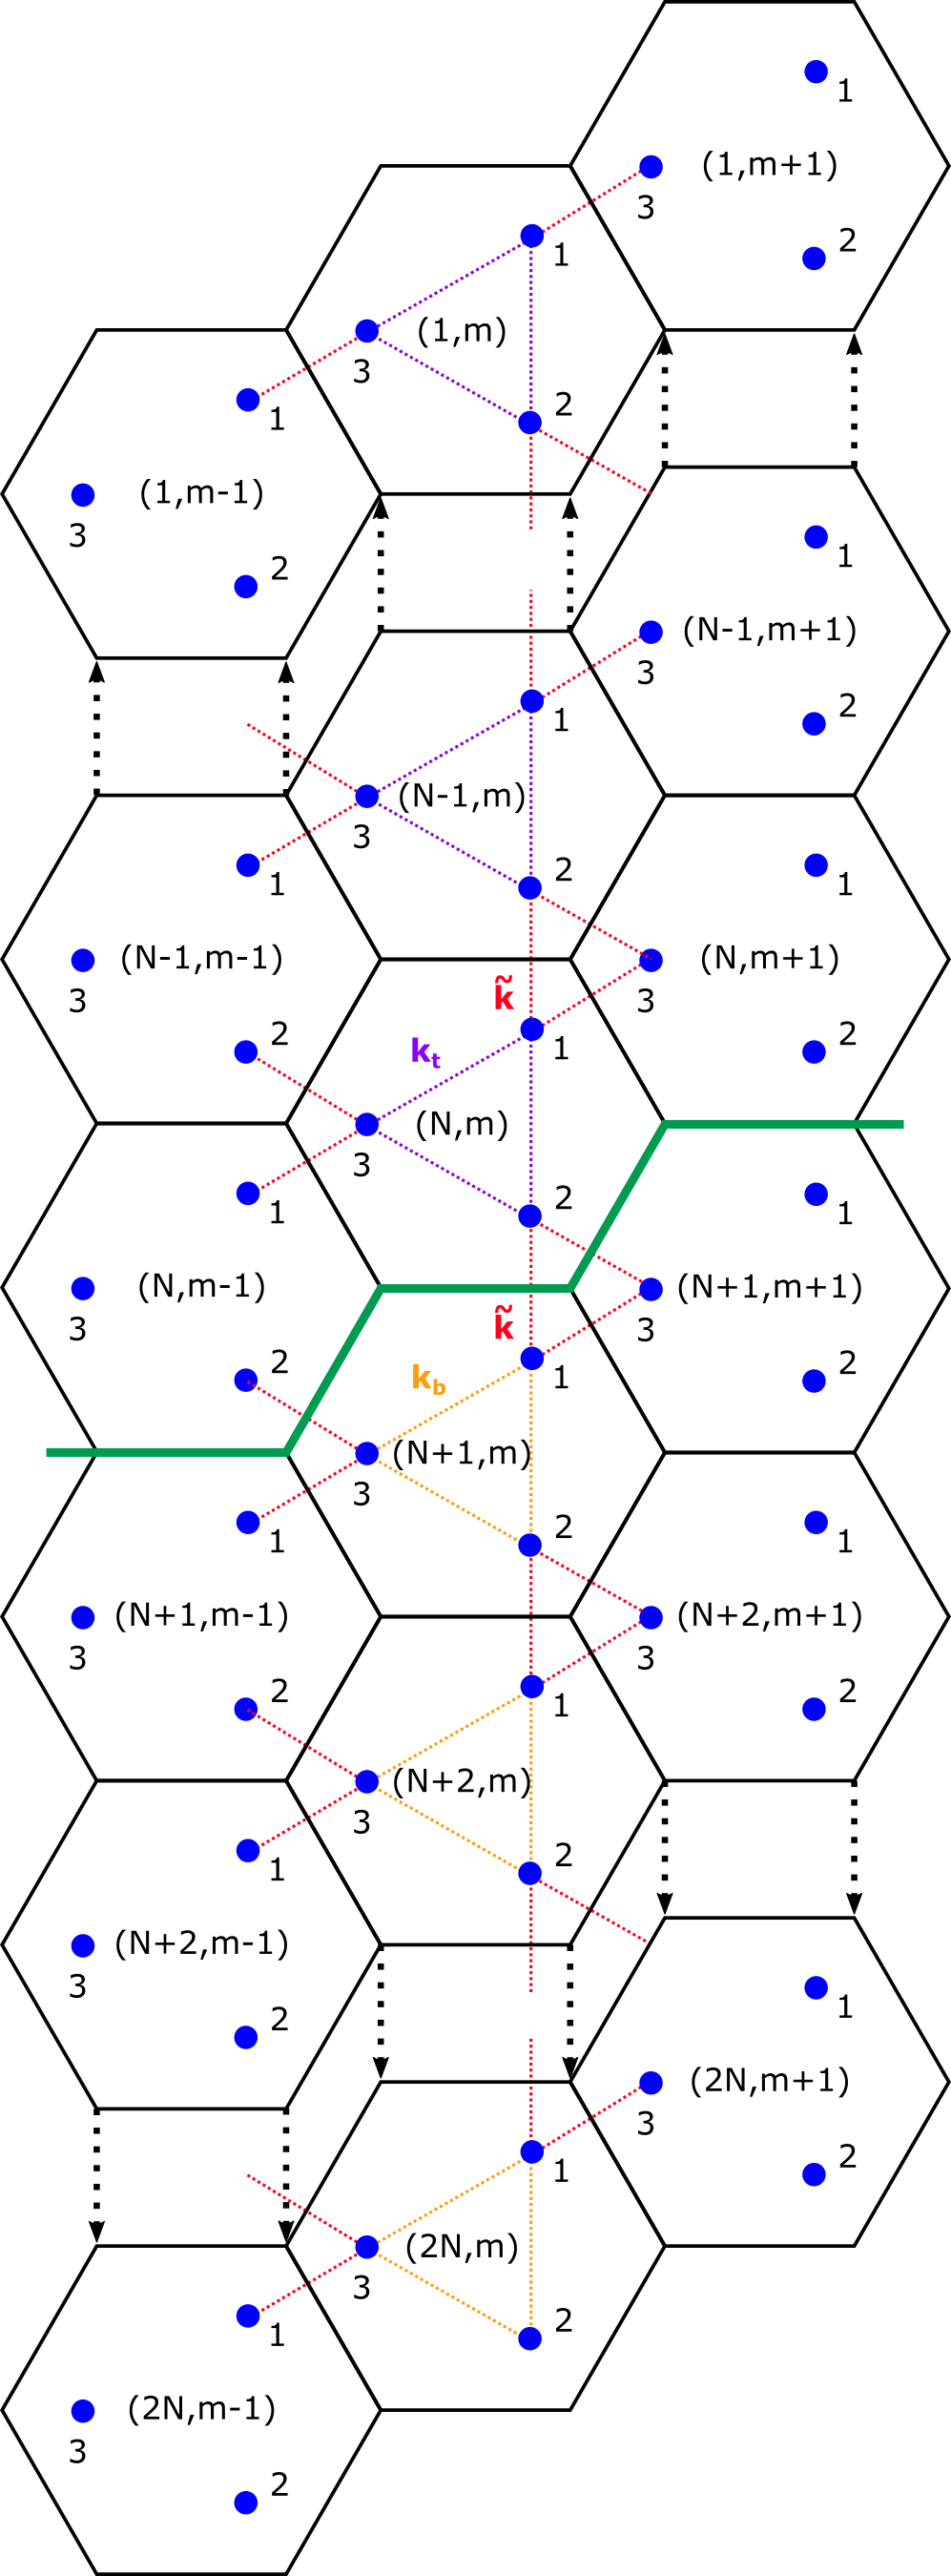
\includegraphics[width=0.4\textwidth]{imgs/kagomestripmodel.png}
\caption{\label{fig:kagomestripmodel} Schematic view of the 2d kagome
  semi-infinite lattice made from an infinite number of strips connected
  side-by-side. Each strip is composed of 2N cells, with the top half of cells
  above the boundary (green) possessing a set of properties and the bottom half
  possessing a separate set of properties.}
\end{figure}

As we have just done in the hexagonal case, we assemble $2N$ kagome cells
together into a strip and form a semi-infinite lattice with these strips
connected left-to-right as shown in Figure~\ref{fig:kagomestripmodel}.

Using the same conventions as the hexagonal strip case and similarly imposing
rigid boundary conditions at the top and bottom edge, we can form the
eigen-problem

%\begin{align}
%  \matr{A}_{1,3(2N-1)+2}&=\matr{A}_{3(2N-1)+2,1}=-\tilde{k} \\
%  \matr{A}_{3,3(2N-1)+2}&=-\tilde{k}e^{-i\Delta_1} \\
%  \matr{A}_{3(2N-1)+2,3}&=-\tilde{k}e^{i\Delta_1} 
%\end{align} 

\begin{align}
  \left[\matr{A}\left(\kappa_{x},\kappa_{y}\right)-\matr{\Omega}\matr{M}\right]\vec{y}=\vec{0}
\label{eq:kagomestripeig}
\end{align}

where $\matr{A}$ is a $(2N \times 6) \times (2N \times 6)$ matrix with
$\matr{A}$ as defined in \eqref{eq:kagomeeig} repeated along the diagonal and
with the additional coupling terms added,
$\matr{\Omega}=\diag\left(\left\{\Omega_i^2\right\}\right)$,
$\matr{M}_{t}=\diag\left(\left\{M_{i,t}\right\}\right)$,
$\matr{M}_{b}=\diag\left(\left\{M_{i,b}\right\}\right)$,
\begin{align}
\matr{M}=\left[
\begin{array}{cccccc}
\matr{M}_{t}\\
 & \ddots &  &  & 0\\
 &  & \matr{M}_{t}\\
 &  &  & \matr{M}_{b}\\
 & 0 &  &  & \ddots\\
 &  &  &  &  & \matr{M}_{b}
\end{array}\right],
\end{align}

\begin{align}
\vec{y}=\left[
\begin{array}{c}
y_1^{(1)}\\
y_2^{(1)}\\
y_3^{(1)}\\
\vdots\\
y_1^{(2N)}\\
y_2^{(2N)}\\
y_3^{(2N)}\\
\end{array}\right],
\end{align}

Solving this with $M_{i,t}=M_{i,b}=k_t=k_b=\tilde{k}=1$ over the irreducible
Brilloun zone, which is again the same as the hexagonal system, gives us the
dispersion relation in Figure~\ref{fig:kagomestripdisper}.

\begin{figure}[!h]
\centering
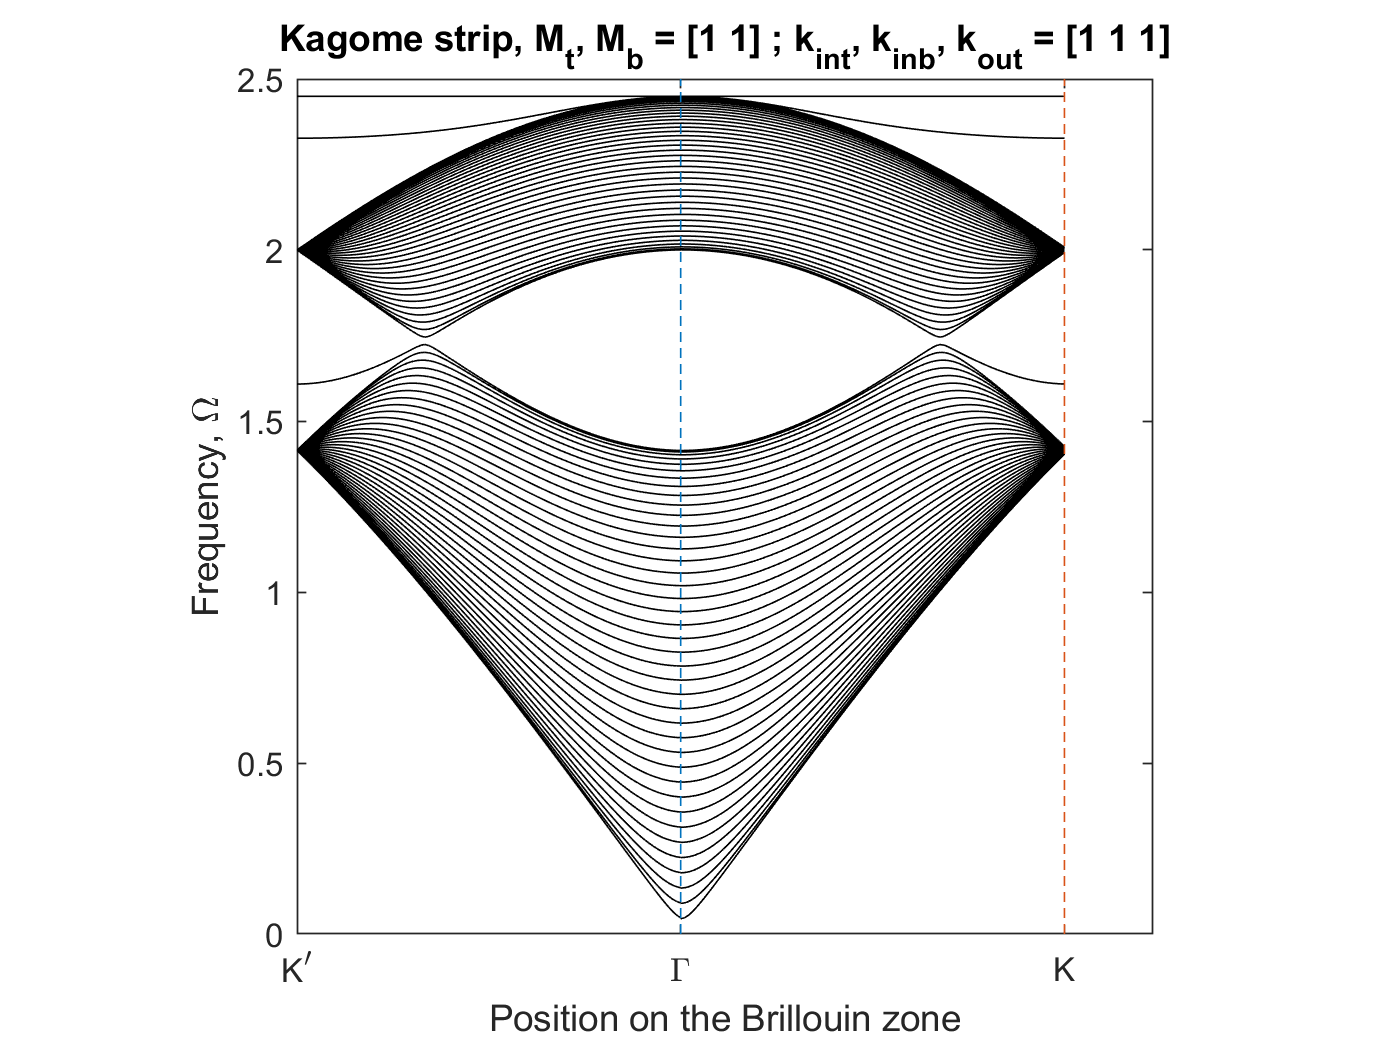
\includegraphics[width=0.8\textwidth]{imgs/kagomestrip.png}
\caption{\label{fig:kagomestripdisper} Dispersion relation of the semi-infinite
  kagome lattice with $2N=40$ (40 cells in total) with
  $M_{i,t}=M_{i,b}=k_t=k_b=\tilde{k}=1$.}
\end{figure}

Now let us try to get the dispersion relation for the semi-infinite kagome
lattice where the top material is made of the kagome cells with increased $M_i$
and $k$ and the bottom material is made of kagome cells decreased $M_i$ and
$k$, as we used in Figure~\ref{fig:kagome2}.

\begin{figure}[!h]
\centering
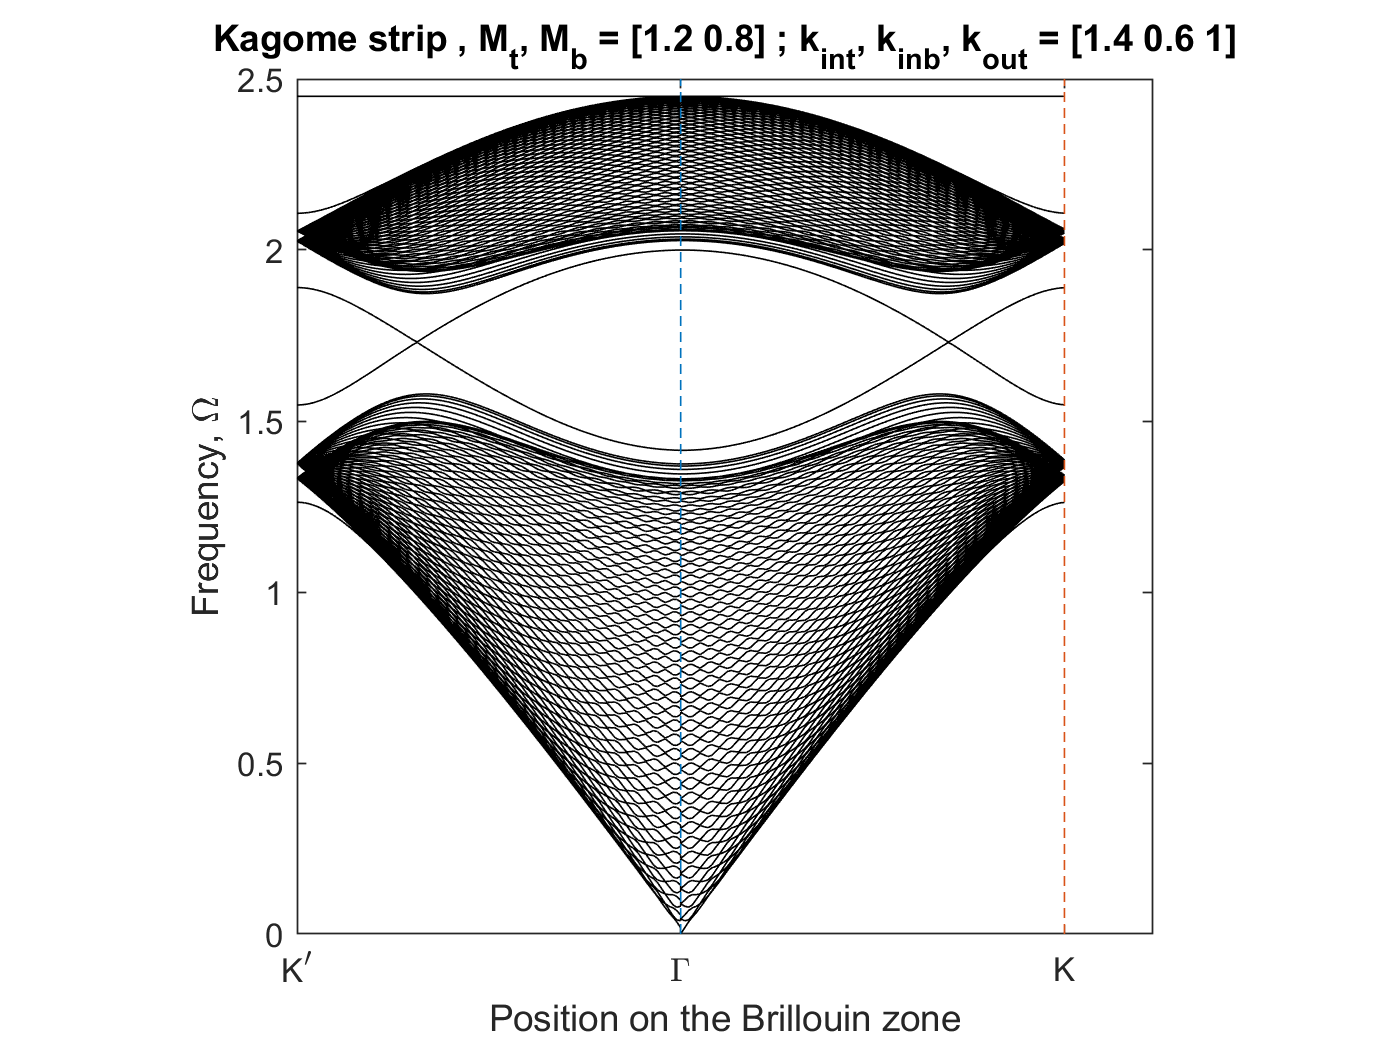
\includegraphics[width=0.8\textwidth]{imgs/kagomestripperturbed.png}
\caption{\label{fig:kagomeperturbed} Dispersion relation of the semi-infinite
  kagome lattice where the top material has a higher $M_i$ and $k$ than the
  bottom material, with all other parameters set to $1$.}
\end{figure}

Again, as in the hexagonal case, we have a bandgap with two well-defined
dispersion curves corresponding to edge states which live on the boundary.
